\documentclass[aspectratio=169,10pt]{beamer}

\usetheme{metropolis}
\usepackage{appendixnumberbeamer}

\usepackage{booktabs}
\usepackage{graphicx}
\usepackage{amsmath, amssymb}
\usepackage{tikz}
\usetikzlibrary{positioning, shapes.geometric, fit, backgrounds, calc, shadows,
    decorations.pathreplacing, arrows.meta}

\usepackage[backend=biber, style=numeric]{biblatex}
\addbibresource{../../refs.bib}

% Figure macros
% LSM-tree figure — \LSMtree command. Toggle filter overlay via \LSMfilterstrue.
% Yellow SSTable cells in pink rounded group boxes, dashed memory/disk separator,
% memtable triangle. Mirrors the proposal-slides style.

\newif\ifLSMfilters
\LSMfiltersfalse

\definecolor{LSMpink}{HTML}{FCE7E5}
\definecolor{LSMpinkEdge}{HTML}{8A6E6A}
\definecolor{LSMyellow}{HTML}{FCEFA1}
\definecolor{LSMyellowEdge}{HTML}{8A8260}
\definecolor{LSMblue}{HTML}{6FA8DC}
\definecolor{LSMblueEdge}{HTML}{3D6FA0}

% \sstgroupblock{prefix}{x_origin}{y_bottom}{ncols_minus_1}
% Cells: (\cx,\cy) at (x_origin + 0.32*cx, y_bottom + 0.32*cy)
\newcommand{\sstgroupblock}[4]{%
    \foreach \cx in {0,...,#4} {
        \foreach \cy in {0, 1} {
            \node[sstcell] (#1-\cx-\cy) at (#2 + 0.32*\cx, #3 + 0.32*\cy) {};
        }
    }
    \begin{scope}[on background layer]
        \node[sstgroup, fit=(#1-0-0)(#1-#4-1)] (#1-box) {};
    \end{scope}
    \ifLSMfilters
        \node[fblob] at (#1-box.north west) {};
    \fi
}

\newcommand{\LSMtree}{%
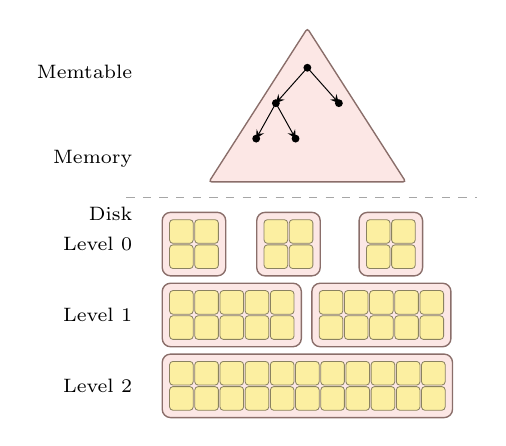
\begin{tikzpicture}[
    sstcell/.style={draw=LSMyellowEdge, line width=0.3pt, rounded corners=1.2pt,
                    fill=LSMyellow, minimum width=0.30cm,
                    minimum height=0.30cm, inner sep=0pt},
    sstgroup/.style={draw=LSMpinkEdge, line width=0.5pt, rounded corners=3pt,
                     fill=LSMpink, inner sep=2.5pt},
    fblob/.style={draw=LSMblueEdge, line width=0.4pt, fill=LSMblue,
                  rounded corners=1pt, minimum size=0.22cm, inner sep=0pt},
    rlabel/.style={font=\scriptsize, anchor=east, text=black},
]

% --- Memtable triangle (centered horizontally over the LSM levels) ---
% Levels span x ∈ [0.20, 3.40]. Center ≈ 1.80.
\coordinate (memtop)  at (1.80, 2.05);
\coordinate (membotL) at (0.55, 0.10);
\coordinate (membotR) at (3.05, 0.10);
\fill[LSMpink, draw=LSMpinkEdge, line width=0.5pt, rounded corners=1pt]
    (memtop) -- (membotR) -- (membotL) -- cycle;
% 5-node binary tree inside the triangle (root + 2 children + 2 grandchildren)
\coordinate (n1) at (1.80, 1.55);    % root
\coordinate (n2) at (1.40, 1.10);    % left child
\coordinate (n3) at (2.20, 1.10);    % right child
\coordinate (n4) at (1.15, 0.65);    % 2's left
\coordinate (n5) at (1.65, 0.65);    % 2's right
\foreach \n in {n1, n2, n3, n4, n5} { \fill (\n) circle (0.05); }
\draw[->, >=stealth, line width=0.35pt] (n1) -- (n2);
\draw[->, >=stealth, line width=0.35pt] (n1) -- (n3);
\draw[->, >=stealth, line width=0.35pt] (n2) -- (n4);
\draw[->, >=stealth, line width=0.35pt] (n2) -- (n5);

% --- Memory/Disk dashed separator ---
\draw[dashed, gray!70, line width=0.5pt] (-0.50, -0.10) -- (3.95, -0.10);

% --- Level 0: 3 groups of 2 cols, bottom row at y = -0.85 ---
\sstgroupblock{l0a}{0.20}{-0.85}{1}
\sstgroupblock{l0b}{1.40}{-0.85}{1}
\sstgroupblock{l0c}{2.70}{-0.85}{1}

% --- Level 1: 2 groups of 5 cols, bottom row at y = -1.75 ---
\sstgroupblock{l1a}{0.20}{-1.75}{4}
\sstgroupblock{l1b}{2.10}{-1.75}{4}

% --- Level 2: 1 group of 11 cols, bottom row at y = -2.65 ---
\sstgroupblock{l2a}{0.20}{-2.65}{10}

% --- Left labels (gap from leftmost cell column at x=0.20) ---
\node[rlabel] at (-0.30, 1.50) {Memtable};
\node[rlabel] at (-0.30, 0.40) {Memory};
\node[rlabel] at (-0.30, -0.30) {Disk};
\node[rlabel] at (-0.30, -0.85+0.16) {Level 0};
\node[rlabel] at (-0.30, -1.75+0.16) {Level 1};
\node[rlabel] at (-0.30, -2.65+0.16) {Level 2};

% (SSTables brace removed — Level 0/1/2 labels carry the meaning;
%  brace + label was making the figure too wide for a half-slide column.)

\end{tikzpicture}%
}

% Hash → ERE pipeline diagram (compact vertical layout for half-slide column).
\newcommand{\HashEREpipeline}{%
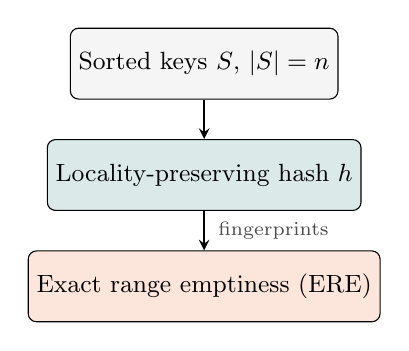
\begin{tikzpicture}[
    box/.style={draw, rounded corners=3pt, fill=black!4, minimum width=3.4cm,
                minimum height=0.9cm, font=\small, align=center, inner sep=3pt},
    arr/.style={->, >=stealth, line width=0.7pt},
    label/.style={font=\scriptsize, text=black!70},
]
\node[box] (keys) {Sorted keys $S$, $|S| = n$};
\node[box, below=0.5cm of keys, fill=thAccent1!15] (hash) {Locality-preserving hash $h$};
\node[box, below=0.5cm of hash, fill=thAccent2!15] (ere)  {Exact range emptiness (ERE)};
\draw[arr] (keys) -- (hash);
\draw[arr] (hash) -- node[label, right=0.05cm] {fingerprints} (ere);
\end{tikzpicture}%
}


% --- Color palette: matches benchmark plots
\definecolor{thScanARE}{HTML}{D946EF}    % magenta — Scan-ARE
\definecolor{thRosetta}{HTML}{12FC21}    % neon green — Rosetta
\definecolor{thSNARF}{HTML}{1E3A8A}      % deep blue
\definecolor{thGrafite}{HTML}{0F766E}    % teal
\definecolor{thAccent1}{HTML}{0F766E}    % teal accent
\definecolor{thAccent2}{HTML}{EA580C}    % orange accent

\setbeamercolor{progress bar}{fg=thAccent1}
\setbeamercolor{title separator}{fg=thAccent2}
\setbeamercolor{frametitle}{bg=black!5, fg=black}
\setbeamerfont{frametitle}{family=\sffamily, series=\bfseries, size=\Large}

% --- Title block
\title{Practical Range Emptiness Filters}
\subtitle{Succinct Backend and a Data-Aware Filter}
\author{Andrei Ogurtsov \\[0.3em] {\footnotesize Supervised by Artem Anisimov}}
\institute{Bachelor's Thesis Defence}
\date{2026}

\begin{document}

\maketitle

%\begin{frame}{Talk in One Sentence}
%  \vspace{1em}
%  \begin{center}
%    \large
%    Non-asymptotic optimizations on three layers $-$\\[0.4em]
%    Layer 3 produces a result \textbf{beyond the original scope}.
%  \end{center}
%  \vspace{1em}
%  \begin{itemize}
%    \item \textbf{Layer 1} $-$ succinct backend (one-vector ERE; WPS $\to$ binary search)
%    \item \textbf{Layer 2} $-$ hash design (truncation + adaptive)
%    \item \textbf{Layer 3} $-$ Scan-ARE (1D-DBSCAN over sorted keys)
%  \end{itemize}
%\end{frame}

% Core slides — all in core/
\begin{frame}{Log-Structured Merge-Tree (LSM Tree)}
  \begin{columns}[T,onlytextwidth]
    \column{0.50\textwidth}
    \begin{itemize}
      \item \textbf{Write-optimized} storage structure
      \item Data is stored in immutable sorted files (\textbf{SSTables})
      \item SSTables are organized into multiple \textbf{levels}
      \item Widely used \\ \emph{(RocksDB, LevelDB, Cassandra, HBase)}
      \item A point lookup requires touching \textbf{every level}
    \end{itemize}

    \column{0.48\textwidth}
    \centering
    \LSMfiltersfalse
    \scalebox{0.95}{\LSMtree}
  \end{columns}
\end{frame}

\begin{frame}{Reducing Disk I/O with Filters}
  \begin{columns}[T,onlytextwidth]
    \column{0.50\textwidth}
    Approximate membership filters answer `Maybe Contains?' queries with False Positives (FPs) allowed --- cutting down disk lookups:
    \begin{itemize}
      \item Filters live in SSTable \textbf{metadata}
      \item Filters use \textbf{small memory} compared to the SSTable itself (10 --- 20 bit per key)
      \item Point queries --- bloom filters
      \item Range queries --- range filters
    \end{itemize}

    \column{0.48\textwidth}
    \centering
    \LSMfilterstrue
    \scalebox{0.95}{\LSMtree}
  \end{columns}
\end{frame}

\begin{frame}{Problem and Goswami Baseline}
  \textbf{Approximate Range Emptiness (ARE).}
  Given a sorted set $S \subseteq [r]$ and query interval $[a, b]$,
  answer ``$S \cap [a, b] = \emptyset$?'' with one-sided error $\varepsilon$:
  no false negatives, $\Pr[\text{false positive}] \leq \varepsilon$.
  \vspace{0.4em}

  \begin{columns}[c,onlytextwidth]
    \column{0.60\textwidth}
    \textbf{Lower bound (Goswami, SODA'15):}
    \[
      \mathrm{BPK} \;\geq\; \log_2\!\left(\frac{n\,\mathcal{L}}{\varepsilon}\right)\Big/\,n
    \]
    Their construction reaches it via:
    \begin{itemize}
      \item \textbf{Locality-preserving hash $h$} --- maps key ranges to
            fingerprint ranges, shrinking the universe to
            $O(n\mathcal{L}/\varepsilon)$.
      \item \textbf{Exact range emptiness (ERE)} --- answers
            ``$S' \cap [a,b] = \emptyset$?'' exactly (no false positives) on
            that small universe.
    \end{itemize}

    \column{0.38\textwidth}
    \centering
    \scalebox{0.85}{\HashEREpipeline}
  \end{columns}

  \vspace{0.6em}
  \begin{center}
    \textit{Asymptotically optimal --- but the constants are large in practice.}
  \end{center}
\end{frame}

\begin{frame}[c]{Exact Range Emptiness as Elias-Fano}
  \begin{center}
    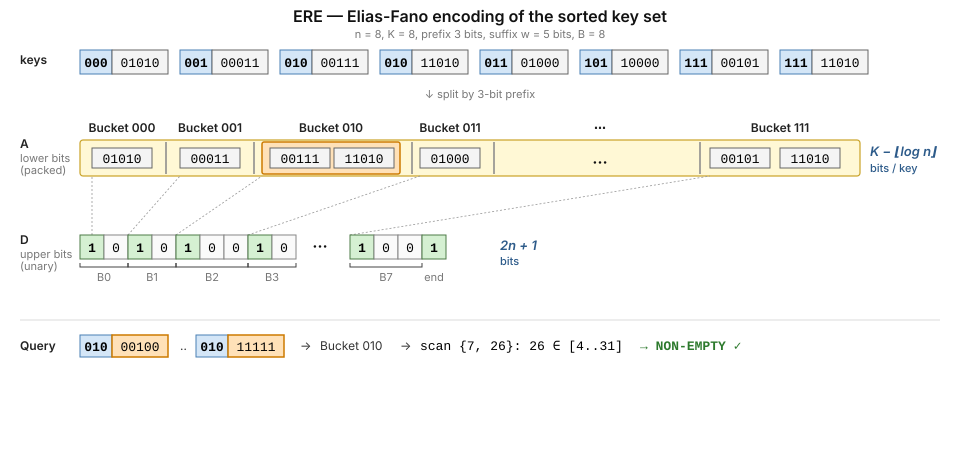
\includegraphics[width=\textwidth, keepaspectratio]{figures/ere_structure_v3}
  \end{center}

  \vspace{-0.8em}
  \textbf{Bucket} $=$ packed array of suffixes for one block;
  $\textsc{Select}(D, i)$ navigates to bucket $i$ in $O(1)$.
\end{frame}

\begin{frame}[c]{Succinct Backend}
    \textbf{Two improvements to the ERE backend.}
    \medskip

    \begin{columns}[T,onlytextwidth]
        \column{0.50\textwidth}
        \begin{itemize}
            \setlength{\itemsep}{0.7em}
            \item \textbf{Navigation:} Goswami two-level metadata $D_1 + D_2\ \to$ one vector $D$\\
                  $-0.80$ bits/key metadata ($\sim\!24\%$)\\
                  $1.1$--$1.9\times$ faster queries

            \item \textbf{Bucket search:} Weak Prefix Search (WPS) $\to$ binary/linear\\
                  ${\ge}\,59$ BPK auxiliary index saved\\
                  \textbf{Speedup: $13$--$30\times$}
        \end{itemize}

        \column{0.5\textwidth}
        \centering
        \footnotesize
        \begin{tabular}{@{}lrrr@{}}
            \toprule
            Dataset                        & Adaptive      & WPS      & $\times$   \\
                                           & Bin./Lin.     &          &            \\
            \midrule
            Facebook median ($k\!=\!27$)   & $10$~ns  & $307$~ns & $30\times$ \\
            Facebook max ($k\!=\!1{,}589$) & $33$~ns  & $514$~ns & $16\times$ \\
            Books median ($k\!=\!812$)     & $20$~ns  & $514$~ns & $26\times$ \\
            Books max ($k\!=\!14{,}039$)   & $43$~ns  & $556$~ns & $13\times$ \\
            \bottomrule
        \end{tabular}
    \end{columns}
\end{frame}
\input{core/07-distributions}
\begin{frame}{Two Regimes: Dense Clusters and Sparse Tails}
    \begin{columns}[T,onlytextwidth]
        \column{0.48\textwidth}
        \textbf{Dense cluster} ($U' = k_{\max} - k_{\min} \ll 2^L$)
        \smallskip
        \begin{itemize}\setlength{\itemsep}{0.35em}
            \item ARE (Goswami): $\;n\log_2(\mathcal{L}/\varepsilon)\;$ bits
                  --- \textbf{independent of $U$}
            \item ERE: $\;n\log_2(U'/n) + O(n)\;$ bits
                  --- \textbf{shrinks with $U'$}
        \end{itemize}
        \medskip
        \begin{center}
            \fbox{$\;U' \le n\mathcal{L}/\varepsilon
                    \;\Longrightarrow\; \text{exact mode,}\ \mathrm{FPR} = 0\;$}
        \end{center}

        \column{0.48\textwidth}
        \textbf{Sparse tail} (wide $U'$, few keys)
        \smallskip
        \begin{center}
            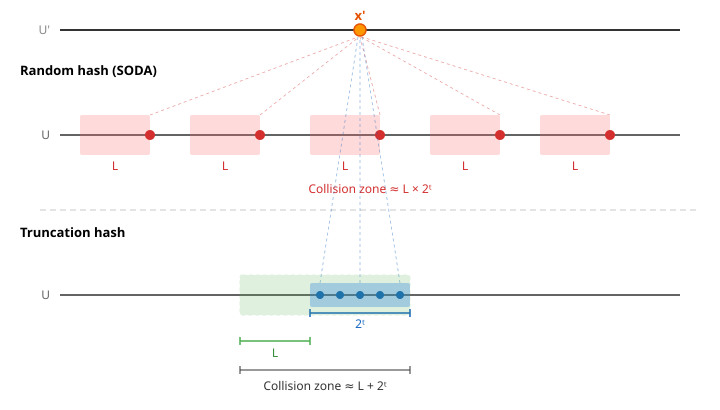
\includegraphics[width=0.92\linewidth, keepaspectratio]{../../figures/phantom_comparison_slide}
        \end{center}
        \begin{itemize}\setlength{\itemsep}{0.2em}
            \item SODA hash:\quad $\log_2(\mathcal{L}/\varepsilon)$ BPK
            \item Truncation:\quad $\log_2(1/\varepsilon)$ BPK
        \end{itemize}
    \end{columns}
\end{frame}

\begin{frame}{Detection: 1D-DBSCAN over Sorted Keys}
    \ourbadge
    \begin{columns}[T,onlytextwidth]
        \column{0.60\textwidth}
        \textbf{Goal:} find segments dense enough to fit exact mode
        at fingerprint width $K = \lceil\log_2(n\mathcal{L}/\varepsilon)\rceil$
        \medskip

        \begin{itemize}
                    \setlength{\itemsep}{0.3em}
                \item One-pass scan over sorted keys, $O(n)$.
                \item DBSCAN (density-based clustering) predicate, radius derived from $K$.
                \item Span $\le 2^K \Rightarrow$ exact ERE (FPR $= 0$);
            else $\Rightarrow$ fallback.
                \item Threshold derived from problem geometry.
        \end{itemize}

        \column{0.40\textwidth}
        \vspace*{3em}
        \centering
        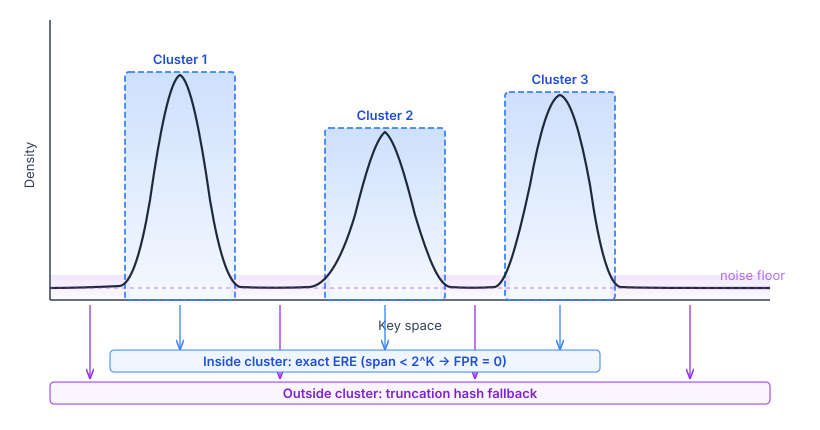
\includegraphics[width=\linewidth, keepaspectratio]{../../figures/segmentation}
        \vspace*{\fill}
    \end{columns}
\end{frame}

\begin{frame}{Headline — SOSD Facebook, $\mathcal{L} = 128$, $n = 2^{24}$}
  \ourbadge
  \centering
  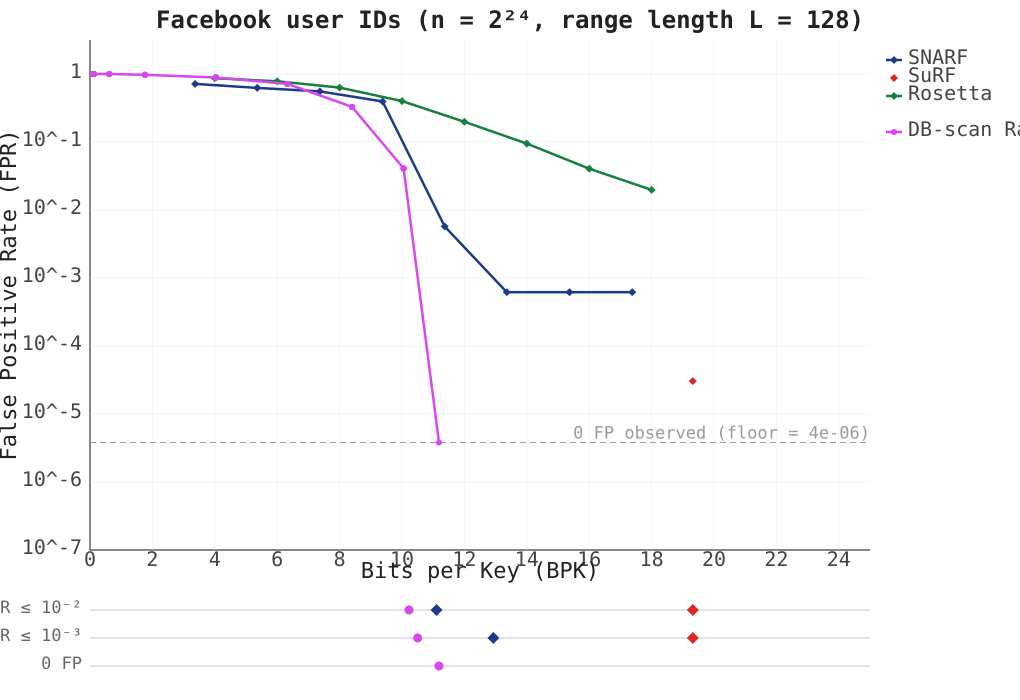
\includegraphics[height=0.78\textheight, keepaspectratio]{figures/headline_fb_L128}

  \vspace{0.3em}
  {\footnotesize
    \textcolor{thScanARE}{\textbf{Segmented-ARE}} hits the 0-FP floor at $\sim 11$ BPK;
    \textcolor{thSNARF}{\textbf{SNARF}} saturates at FPR $\approx 7 \cdot 10^{-4}$.
  }
\end{frame}

\begin{frame}{Limitations — Uniform, $\mathcal{L} = 1$, $n = 2^{24}$}
  \ourbadge
  \begin{columns}[T,onlytextwidth]
    \column{0.6\textwidth}
    \centering
    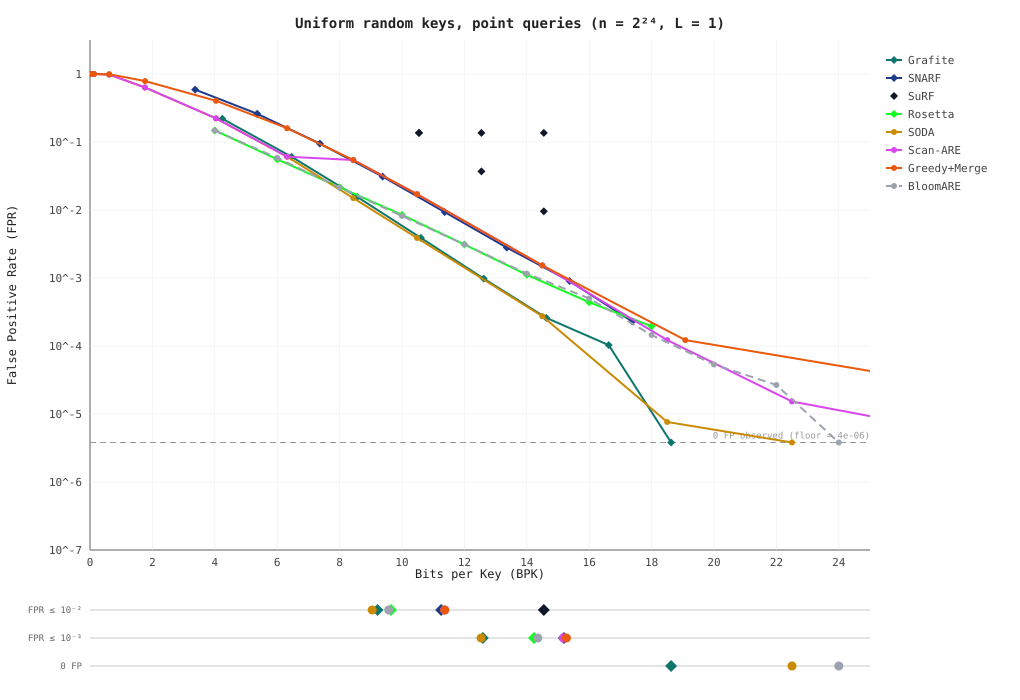
\includegraphics[width=\linewidth, keepaspectratio]{figures/limitations_uniform_L1}

    \column{0.42\textwidth}
    \textbf{Where we lose.}
    \begin{itemize}
      \item No clusters $\Rightarrow$ segmentation gives no advantage.
      \item No range $\Rightarrow$ truncation gives no advantage.
    \end{itemize}
    \vspace{0.4em}
    \emph{Honest reading:} on uniform + point queries, the industry baseline wins.
    \\ We gain a lot on clustered data.
  \end{columns}
\end{frame}

\begin{frame}{Conclusion — Three Results}
  \begin{columns}[c,onlytextwidth]
    \column{0.32\textwidth}
    \centering
    {\Huge\bfseries\textcolor{thAccent1}{$-24\%$}}\\[0.4em]
    {\small metadata bits}\\
    {\footnotesize Layer 1 — one-vector ERE}

    \column{0.32\textwidth}
    \centering
    {\Huge\bfseries\textcolor{thAccent2}{$8$--$160\times$}}\\[0.4em]
    {\small WPS $\to$ binsearch}\\
    {\footnotesize Layer 1 — query latency}

    \column{0.32\textwidth}
    \centering
    {\Huge\bfseries\textcolor{thScanARE}{$<\!10^{-8}$}}\\[0.4em]
    {\small at $\sim 11$ BPK}\\
    {\footnotesize Layer 3 — Scan-ARE on Facebook user IDs}
  \end{columns}
  \vspace{1em}
  \centering
  \emph{Non-asymptotic optimizations on three layers.}\\
  \vspace{0.4em}
  {\footnotesize End-to-end query latency on Facebook user IDs: see appendix.}\\
  \vspace{0.3em}
  {\footnotesize Future work: RocksDB integration, other clustering approaches.}
\end{frame}


\appendix
% DLC modules — load conditionally
% \input{dlc/M1-onevector}
% \input{dlc/M2-adaptive}
% \input{dlc/M3-lsm-context}
% \input{dlc/M4-industry-comparison}

% Backup slides — Q&A
\begin{frame}{Backup --- Query Latency on Mostly-Negative Queries}
  \centering
  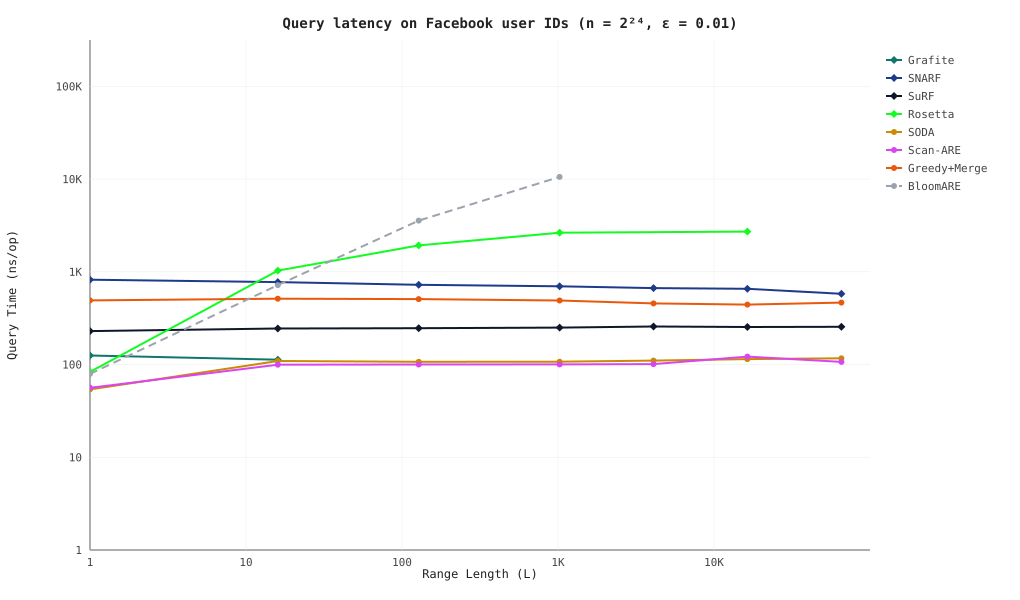
\includegraphics[height=0.72\textheight, keepaspectratio]{figures/latency_fb_gap_heavy}

  \vspace{0.2em}
  {\footnotesize
    Facebook user IDs, $n = 2^{24}$, $\varepsilon = 10^{-2}$, mostly-negative queries.
    \textcolor{thScanARE}{\textbf{Segmented-ARE}} $\sim\!100$\,ns flat;
    \textcolor{thSNARF}{\textbf{SNARF}} $\sim\!700$\,ns;
    \textcolor{thRosetta}{\textbf{Rosetta}} $\to 2500\,$ns at $\mathcal{L}{=}4096$;
  }
\end{frame}


\end{document}
